% main.tex - Main file that imports all sections
\documentclass[12pt,a4paper,twoside]{report} %12pt -> font size as requested by uni guidelines

% Packages
\usepackage[T1]{fontenc}
\usepackage{lmodern}
\usepackage[utf8]{inputenc}
\usepackage[main=italian, english]{babel}
\usepackage[top=3cm, bottom=3cm, left=3cm, right=3cm]{geometry}
\usepackage{graphicx}  % For images
\usepackage{booktabs}  % For professional tables
\usepackage{amsmath,amssymb}  % For math
\usepackage[numbers]{natbib}    % For bibliography
\usepackage{fancyhdr} % For headers and footers
\usepackage{setspace} % For "interlinea"
\usepackage{hyperref}
\graphicspath{{images/}}



\setlength{\headheight}{27.2pt}
\addtolength{\topmargin}{-12.62pt}



\newcommand{\universityname}{Università degli Studi di Bergamo}
\newcommand{\facultyname}{Scuola di Ingegneria}
\newcommand{\departmentname}{Dipartimento di Ingegneria Gestionale, dell'Informazione e della Produzione}
\newcommand{\coursename}{Corso di Laurea Magistrale in Ingegneria Informatica}
\newcommand{\courseclass}{Classe n.~LM-32 -- Ingegneria Informatica}
\newcommand{\thesistitle}{Titolo vero della tesi}
\newcommand{\thesisauthor}{Federico Panzeri}
\newcommand{\studentid}{123456}               
\newcommand{\academicyear}{2025/2026}           
\newcommand{\supervisorname}{Chiar.mo Prof.~Mirko Mazzoleni}
\newcommand{\cosupervisorname}{eventuale correlatore}             

% Page styles
\pagestyle{fancy}
\fancyhf{}
\fancyhead[LE,RO]{\thepage}
\fancyhead[LO]{\leftmark}
\fancyhead[RE]{\rightmark}

% posizionamento tabella in pagina vuota
\makeatletter
\setlength{\@fptop}{0pt}
\makeatother

\begin{document}

% Title page
% Frontespizio
\begin{titlepage}
    \centering
    \Large\textbf{\universityname}\\
    \vspace{0.5cm}
    \large \departmentname\\
    \vspace{0.5cm}
    \large \coursename\\
    \courseclass

    \vspace{1cm}
    
\includegraphics[width=5cm]{UNIBG_logo.jpg}\\[0.5cm]
    {\Huge\textbf{\thesistitle}\par}

    \vspace{1cm}

    \begin{flushleft}
        \large
        Relatore:\\
        \supervisorname\\[0.5cm]

        Correlatore:\\
        \cosupervisorname
    \end{flushleft}

    \vfill

    \begin{flushright}
        \normalsize\textbf{Tesi di Laurea Magistrale}\\[0.5cm]
        \normalsize \thesisauthor\\
        \large Matricola n.~\studentid
    \end{flushright}

    \normalsize Anno Accademico \academicyear
\end{titlepage}


% Set 1,5 spacing for the rest of the document
\onehalfspacing% Front matter
\clearpage % force a page break
\pagenumbering{roman}

% Abstract/Summary
% sections/frontmatter/abstract.tex
\begin{abstract}
    Riassunto di quanto svolto, da fare alla fine
\end{abstract}

% Table of contents
\tableofcontents
\listoffigures
\listoftables
\clearpage

% Main stuff
\pagenumbering{arabic}

% Introduction
% sections/introduction.tex
\chapter{Introduction}
\label{chap:introduction}

\section{Sezione 1}
L’Automatic Identification System (AIS) è un sistema di trasmissione e ricezione dati sviluppato da Benny Pettersson agli inizi
degli anni '90 che viene utilizzato in maniera diffusa sia da imbarcazioni commerciali che da diporto. 
Tale dispositivo nasce originariamente con lo scopo di migliorare la sicurezza della navigazione attraverso la riduzione 
del rischio di collisioni; successivamente, con l'evolversi della tecnologia, assume anche un ruolo legato al tracciamento
delle imbarcazioni.
Al di là di queste finalità operative, l’AIS rappresenta oggi una fonte ricca di informazioni per lo studio dei comportamenti 
dei natanti: fornisce dati geolocalizzati (con frequenza temporale variabile ma comunque nell'ordine delle decine di secondi) 
che descrivono in dettaglio i percorsi seguiti dalle navi, la loro velocità, orientamento, stato di navigazione 
e altre caratteristiche sia statiche che dinamiche.

Grazie alla larga adozione del sistema AIS, e grazie anche all'elevata frequenza con cui i dati vengono trasmessi,
è naturale che negli ultimi anni, anche in aree circoscritte ma sufficientemente trafficate, vengano generate grandi moli 
di dati AIS. Tuttavia, la vastità, rumorosità e complessità intrinseca di questi dataset rendono necessario l'impiego di diverse 
tecniche per estrarre informazioni utili. Tutto ciò ha quindi favorito lo sviluppo di diversi studi dedicati all'estrazione 
automatica di informazioni.

L’obiettivo della presente tesi si inserisce in questo contesto: partendo da un metodo di anomaly detection proposto in letteratura,
 esso viene analizzato, migliorato e applicato a un dataset AIS di grandi dimensioni. Prima di descrivere il lavoro svolto, 
 è necessario delineare il quadro delle principali categorie di approcci esistenti, 
 con particolare riferimento ai contributi discussi da Wolsing et al. nel loro lavoro di rassegna e al framework introdotto da 
 Pallotta et al., da cui prende avvio il metodo adottato in questa tesi.

\section{Thesis Structure}
Struttura della tesi.
\begin{itemize}
    \item Chapter \ref{chap:literature} 
    \item Chapter \ref{chap:methodology} 
    \item Chapter \ref{chap:results} 
    \item Chapter \ref{chap:conclusions} 
\end{itemize}

% Literature Review
% sections/literature_review.tex
\chapter{Literature Review}
\label{chap:literature}

% ─────────────────────────────────────────────
\section{Contesto della tesi}
\label{sec:contesto}


L’obiettivo di questa literature review è quello di esplorare lo stato dell’arte delle tecniche 
di analisi dei dati AIS per il rilevamento di anomalie nel traffico marittimo, 
cercando di fornire una panoramica generale.

\subsection{Storia e funzionamento dell'AIS}

L’Automatic Identification System (AIS) è un sistema di comunicazione utilizzato nella navigazione marittima. 
La sua origine viene generalmente attribuita a Benny Pettersson, che sviluppò un primo prototipo nei primi anni 
’90. Inizialmente concepito per ridurre il rischio di collisioni in mare, il sistema è stato poi 
progressivamente adottato a livello internazionale, fino a ottenere un riconoscimento formale da parte 
dell’International Maritime Organization (IMO). 
Nell’ambito dell’accordo SOLAS, l’installazione dell’AIS è diventata obbligatoria per le navi con 
stazza lorda superiore a 300 tonnellate impegnate in viaggi internazionali e per tutte le navi passeggeri 
\cite{imo2002}.

Dal punto di vista tecnico, l’AIS opera su due canali radio VHF intorno ai 162 MHz 
e utilizza il protocollo TDMA (Time-Division Multiple Access), 
che permette a più imbarcazioni di trasmettere senza interferire tra loro \cite{riassuntone}. 
La copertura, in condizioni standard, arriva fino a circa 50 km (linea di vista), 
mentre l’uso di ricevitori satellitari (S-AIS) consente di estenderla anche alle acque oceaniche \cite{riassuntone}.
 La frequenza di trasmissione dei messaggi non è costante, ma varia in funzione della velocità e dello stato 
 della nave, passando da pochi secondi a diversi minuti \cite{riassuntone}.

\subsection{Dati trasmessi}

I messaggi AIS possono essere suddivisi in tre categorie principali \cite{riassuntone}:

\begin{itemize}
\item \textbf{Dati statici}: includono informazioni identificative della nave, come MMSI, nome, tipo e dimensioni.
\item \textbf{Dati dinamici}: descrivono lo stato corrente della navigazione, tra cui posizione GPS, velocità (SOG), rotta (COG), orientamento della prua (HE), variazione della rotta (ROT) e stato operativo.
\item \textbf{Dati di viaggio}: comprendono informazioni aggiuntive come pescaggio, tipo di carico, destinazione ed ETA. Essendo inseriti manualmente, risultano generalmente meno affidabili \cite{pallotta}.
\end{itemize}

Ai fini dell’analisi del comportamento delle navi, i dati dinamici sono in genere i più rilevanti, 
in quanto descrivono in modo continuo l’evoluzione delle traiettorie.

\subsection{Limiti e problemi noti}

Nonostante la ricchezza informativa, i dati AIS presentano diverse criticità che ne complicano l’analisi. 
Dal punto di vista della qualità, possono verificarsi lacune nella copertura dovute a limiti dei ricevitori 
terrestri o a interferenze, soprattutto in aree molto trafficate \cite{pallotta}.

Inoltre, il protocollo AIS non prevede meccanismi di autenticazione o cifratura, 
rendendo possibile la manipolazione dei dati, ad esempio tramite spoofing o spegnimento del transponder \cite{riassuntone}. 
Un ulteriore problema è rappresentato dalla diversa frequenza di trasmissione tra le varie classi di 
imbarcazioni, che introduce una certa eterogeneità nei dataset.

Nel complesso, la dimensione, la rumorosità e la complessità di questi dati rendono necessario 
l’utilizzo di tecniche automatiche di analisi dei dati.

% ─────────────────────────────────────────────
\section{Panoramica degli approcci di anomaly detection}
\label{sec}

La letteratura sull’anomaly detection nei dati AIS è stata raccolta, ad esempio, in \cite{riassuntone}, 
che prende in esame diversi contributi pubblicati tra il 2007 e il 2021. Un elemento ricorrente è la 
distinzione tra una fase iniziale di modellazione del traffico normale e una successiva fase di 
individuazione delle anomalie.

Le tecniche proposte vengono generalmente suddivise in tre macro-categorie: 
\textbf{Machine Learning}, \textbf{Stocastici} e \textbf{Geometrici}, 
a cui si aggiungono approcci ibridi che combinano più metodologie.

Per quanto riguarda la tipologia di anomalie, si fa riferimento alla classificazione proposta da Lane et al. 
\cite{lane2010}, che distingue diverse forme di comportamento anomalo. 
Tra queste, la più studiata è la \textit{route deviation}, che rappresenta anche il focus del presente lavoro.

\subsection{Approcci di Machine Learning}

Gli approcci basati su machine learning comprendono principalmente metodi di clustering e reti neurali. 
Tra i primi, DBSCAN è particolarmente diffuso, in quanto si adatta bene alla natura spaziale dei dati e 
consente di identificare cluster senza specificarne a priori il numero \cite{pallotta}. 
Le traiettorie che non appartengono ad alcun cluster vengono generalmente considerate anomale.

Le reti neurali, invece, permettono di modellare relazioni più complesse e non lineari, 
e nelle versioni più recenti hanno mostrato buone prestazioni.

Questi approcci risultano scalabili e relativamente semplici da implementare, 
ma presentano anche alcuni limiti, tra cui la scarsa interpretabilità (soprattutto per le reti neurali) 
e la difficoltà di generalizzazione a contesti geografici diversi \cite{mascaro}.

\subsection{Approcci Stocastici}

Gli approcci stocastici modellano il comportamento delle navi come un processo probabilistico. 
Tra le tecniche più comuni si trovano GMM, KDE, Gaussian Process e reti bayesiane.

In generale, questi metodi stimano la distribuzione delle traiettorie normali a partire dai dati storici e 
classificano come anomale quelle con bassa probabilità. 
Offrono una buona base teorica e permettono di quantificare l’incertezza, ma possono risultare onerosi 
dal punto di vista computazionale su dataset molto grandi.

Alcuni lavori, come \cite{kowalska}, mostrano l’efficacia dei Gaussian Process, 
mentre le reti bayesiane risultano interessanti per la loro maggiore interpretabilità, 
pur presentando difficoltà di scalabilità \cite{mascaro}.

\subsection{Approcci Geometrici}

Gli approcci geometrici si basano sulle proprietà spaziali delle traiettorie, 
ad esempio tramite il calcolo del convex hull (inviluppo convessp) delle rotte osservate \cite{riassuntone}. 
Si tratta in genere di metodi semplici e interpretabili, ma meno flessibili e meno robusti in presenza di 
rumore rispetto ad altri approcci.

% ─────────────────────────────────────────────
\section{Il framework TREAD di Pallotta et al.}
\label{sec}

Tra gli approcci presenti in letteratura, il metodo adottato in questo lavoro è il framework TREAD 
(Traffic Route Extraction and Anomaly Detection) proposto da \cite{pallotta}, 
che combina tecniche di clustering e analisi statistica.

Il framework è non supervisionato e incrementale: apprende i pattern di traffico direttamente dai dati AIS 
senza richiedere informazioni preliminari. Il processo si articola in due fasi principali. 
Nella prima fase, vengono identificati i waypoint caratteristici (come porti o punti di passaggio) 
tramite un algoritmo di clustering basato su DBSCAN. Tali waypoint vengono usati per costruire le rotte, definite
come il percorso di un nave da un waypoint di partenza a uno di arrivo. Talvolta waypoint di partenza e di arrivo coincidono.

Nella seconda fase, le rotte apprese vengono utilizzate per analizzare nuove traiettorie e 
individuare eventuali anomalie, sulla base della loro probabilità rispetto al modello.

Tra i principali vantaggi di questo approccio vi sono la possibilità di aggiornare il modello in modo 
incrementale, la capacità di gestire dati AIS anche non continui e una rappresentazione relativamente 
compatta del traffico, adatta anche a dataset di grandi dimensioni.

% Methodology
% sections/methodology.tex
\chapter{Metodologia}\label{chap:methodology}


\section{Introduzione}\label{sec:meth_intro}

Questo capitolo descrive in dettaglio il lavoro svolto per analizzare,
re-implementare ed estendere il framework TREAD di Pallotta
et al.~\cite{pallotta}, applicandolo a un dataset AIS reale relativo
all'arcipelago delle Hawaii.

Come anticipato nel Capitolo~\ref{chap:literature}, il framework TREAD
è stato scelto come punto di partenza in quanto combina un approccio non
supervisionato e incrementale con una rappresentazione compatta del
traffico, caratteristiche che lo rendono adatto all'analisi di dataset
di grandi dimensioni. Il lavoro non si limita a una replica dell'algoritmo
originale, ma ne valuta criticamente l'applicabilità a un contesto più
moderno e voluminoso, identificando gli aspetti mantenuti, quelli adattati
e le eventuali possibilità di miglioramento.

La pipeline implementata si articola in tre fasi principali:
\textbf{pre-processing} dei dati grezzi, \textbf{Knowledge Discovery}
per l'identificazione dei waypoint e l'estrazione delle rotte tramite
clustering, e \textbf{anomaly detection} basata su un modello
probabilistico (KDE e distribuzione di Weibull).

Le sezioni seguenti descrivono ciascuna fase nel dettaglio, a partire
dalla descrizione del dataset utilizzato.

\section{Obiettivi}\label{sec:meth_objectives}

I quesiti di ricerca su cui è stata sviluppata la metodologia sono i seguenti:
\begin{enumerate}
    \item Il framework TREAD (che è stato sviluppato agli inizi degli anni 2010), è ancora applicabile ad un dataset
          moderno e più voluminoso?
    \item Quali aspetti e caratteristiche dell'algoritmo sono ``riciclabili'' e quali hanno richiesto adattamenti o sostituzioni?
    \item È possibile ottenere risultati qualitativamente migliori?
    \item Quali metriche è opportuno utilizzare per quantificare le prestazioni dell'algoritmo?
\end{enumerate} 

\section{Dataset}\label{sec:meth_dataset}

I dati utilizzati provengono dal portale pubblico del NOAA\footnote{Il NOAA mette a disposizione due modalità di accesso ai dati: tramite il portale \url{https://marinecadastre.gov/accessais/}, che consente di filtrare per zona geografica e intervallo temporale, oppure tramite \url{https://hub.marinecadastre.gov/pages/vesseltraffic}, 
che offre il download in bulk di tutti i dati AIS registrati suddivisi per anno.} (National Oceanic and Atmospheric Administration), un'agenzia scientifica e
normativa statunitense con diversi compiti tra cui il monitoraggio oceanico~\cite{noaa_wiki}.
I file scaricati dalla piattaforma hanno nome nel formato \texttt{AIS\_YYYY\_MM\_DD} (dove YYYY rappresenta l'anno, MM il mese e DD il giorno
di registrazione dei dati) e contengono tutti i messaggi ricevuti dall'ente in una singola giornata di tutto il territorio nazionale monitorato.
Per questa tesi sono stati utilizzati i dati relativi al periodo gennaio-marzo 2019 (estremi inclusi), filtrati
sull'area delle Hawaii tramite una bounding box le cui estremità hanno le seguenti coordinate:
\begin{itemize}
    \item Latitudine: da $18.77^\circ$N a $22.63^\circ$N,
    \item Longitudine: da $160.11^\circ$W a $154.39^\circ$W.
\end{itemize}

La figura~\ref{fig:NOAA_selection} mostra un passaggio della fase di scaricamento dei dati dal portale del NOAA\@. 
Si può vedere su mappa il rettangolo descritto dalle coordinate di latitudine e longitudine di cui sopra.

\begin{figure}[htbp]
    \centering
    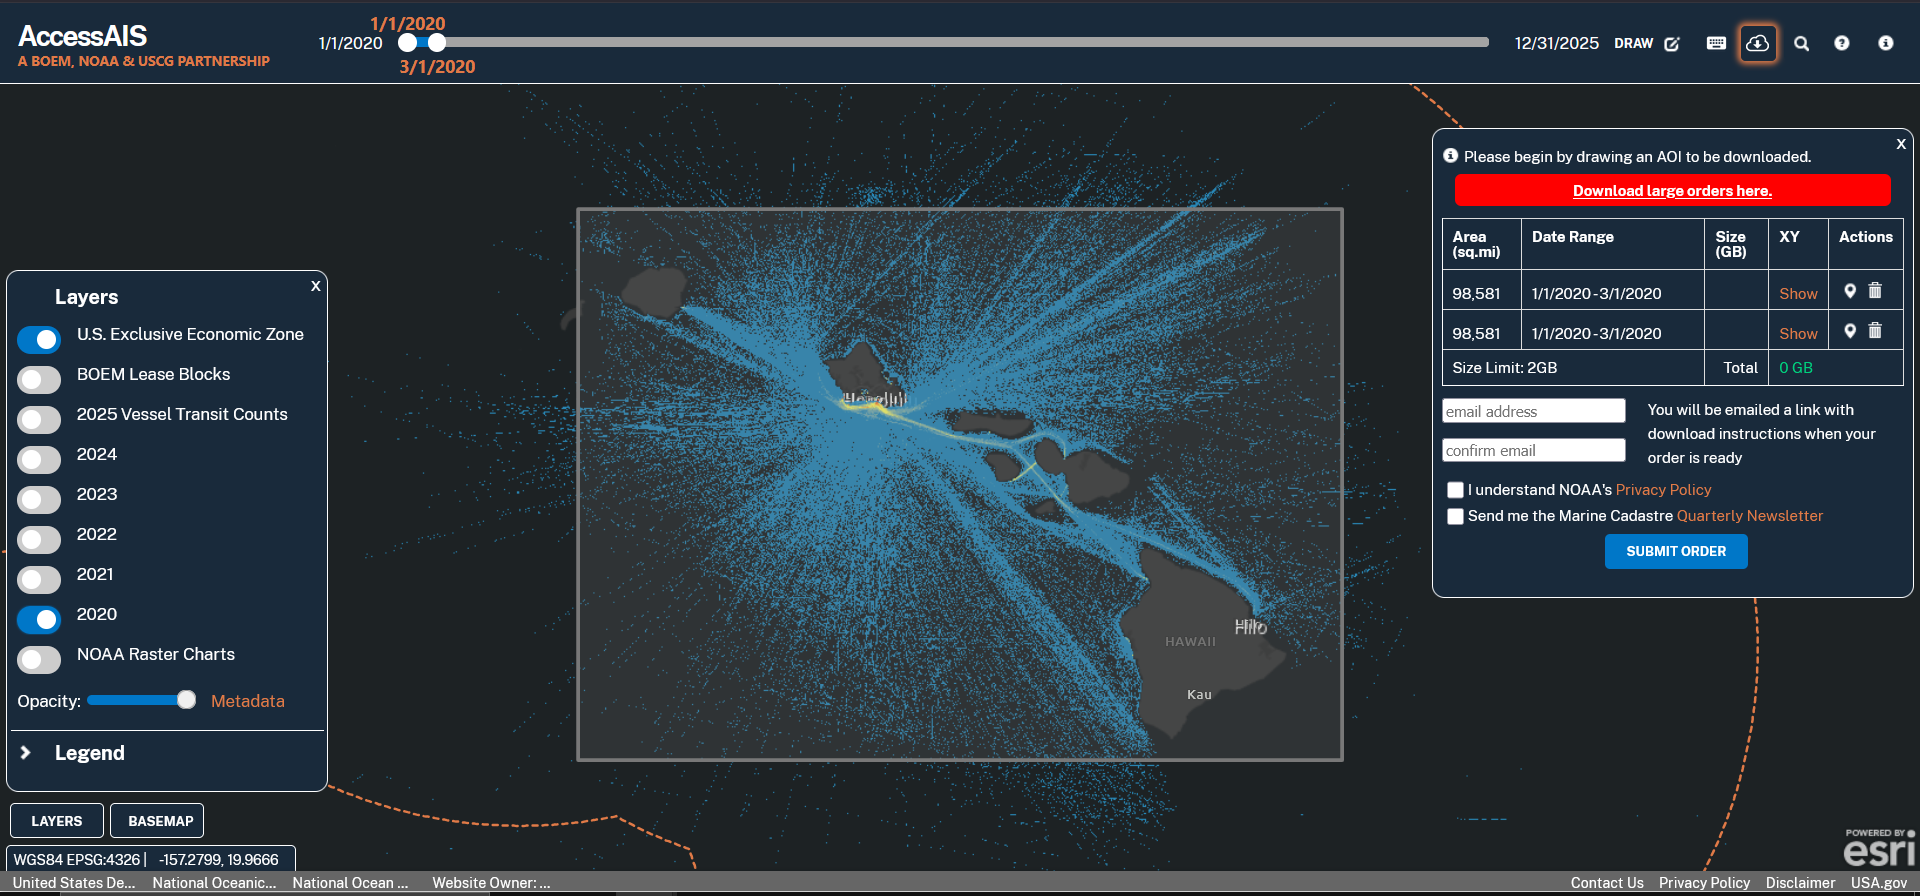
\includegraphics[width=\textwidth]{Methodology/NOAA_AIS_square.PNG}
    \caption{Portale NOAA \textit{AccessAIS} per il download di dati AIS.}\label{fig:NOAA_selection}
\end{figure}

\subsection{Struttura del dataset}\label{ssec:meth_dataset_structure}

Ogni record del dataset corrisponde a un singolo messaggio AIS trasmesso da una nave e contiene diversi campi, riportati nella tabella~\ref{tab:dataset_columns}.
I campi si dividono in due categorie: attributi statici, che descrivono le caratteristiche fisse della nave e normalmente non variano tra
un messaggio e l'altro, e attributi dinamici, che riflettono lo stato corrente della nave al momento della trasmissione.

\begin{table}[htbp]
\centering
\caption{Struttura del dataset AIS del NOAA.}\label{tab:dataset_columns}
\begin{tabular}{llp{7cm}}
\toprule
\textbf{Colonna} & \textbf{Tipo} & \textbf{Descrizione} \\
\midrule
\multicolumn{3}{l}{\textit{Attributi statici}} \\
\texttt{MMSI}          & intero   & Maritime Mobile Service Identity: identificativo univoco della nave \\
\texttt{VesselName}    & stringa  & Nome della nave \\
\texttt{IMO}           & stringa  & Numero IMO (International Maritime Organization) \\
\texttt{CallSign}      & stringa  & Nominativo radio della nave \\
\texttt{VesselType}    & intero   & Codice numerico che indica la tipologia di nave (cargo, tanker, passeggeri, ecc.) \\
\texttt{Length}        & intero   & Lunghezza della nave in metri \\
\texttt{Width}         & intero   & Larghezza della nave in metri \\
\texttt{Draft}         & decimale & Pescaggio della nave in decimi di metro \\
\texttt{Cargo}         & intero   & Codice del tipo di carico trasportato \\
\texttt{TransceiverClass} & booleano & Classe del transponder AIS:\ \texttt{A} o \texttt{B} (imbarcazioni minori) \\
\midrule
\multicolumn{3}{l}{\textit{Attributi dinamici}} \\
\texttt{BaseDateTime}  & datetime & Timestamp del messaggio (UTC) \\
\texttt{LAT}           & decimale & Latitudine della posizione (gradi decimali) \\
\texttt{LON}           & decimale & Longitudine della posizione (gradi decimali) \\
\texttt{SOG}           & decimale & Speed Over Ground: velocità rispetto al fondale in nodi \\
\texttt{COG}           & decimale & Course Over Ground: direzione di movimento in gradi (0--360°) \\
\texttt{Heading}       & decimale & Prua della nave in gradi (0--360°), distinta dal COG \\
\texttt{Status}        & intero   & Stato di navigazione AIS (es.\ in navigazione, all'ancora, in manovra) \\
\bottomrule
\end{tabular}
\end{table}

Ogni record del dataset, contenendo una coppia di coordinate geografiche (\texttt{LAT}, \texttt{LON}),
è rappresentabile come un punto su una mappa. A ciascun punto è inoltre associato un vettore:
il modulo corrisponde alla velocità istantanea della nave (\texttt{SOG}), mentre la direzione è determinata
dall'angolo \texttt{COG}, espresso in gradi rispetto al nord geografico. Questa rappresentazione vettoriale 
è alla base delle elaborazioni descritte nelle sezioni successive, ed è il motivo per cui
nel resto del capitolo i termini \emph{record} e \emph{punto} vengono usati in modo intercambiabile.

In figura~\ref{fig:ais_vessel_diagram} viene mostrata una visualizzazione grafica dei concetti di 
LON, LAT, SOG, COG, Heading. Ogni punto è identificato dalla coppia di coordinate (LON, LAT). 
Il vettore SOG indica la velocità istantanea della nave, con direzione data dall'angolo COG 
misurato rispetto al nord geografico in senso orario. 
L'Heading indica l'orientamento della prua, che può differire dal COG a causa 
di correnti, vento o altre cause



\begin{figure}[htbp]
    \centering
    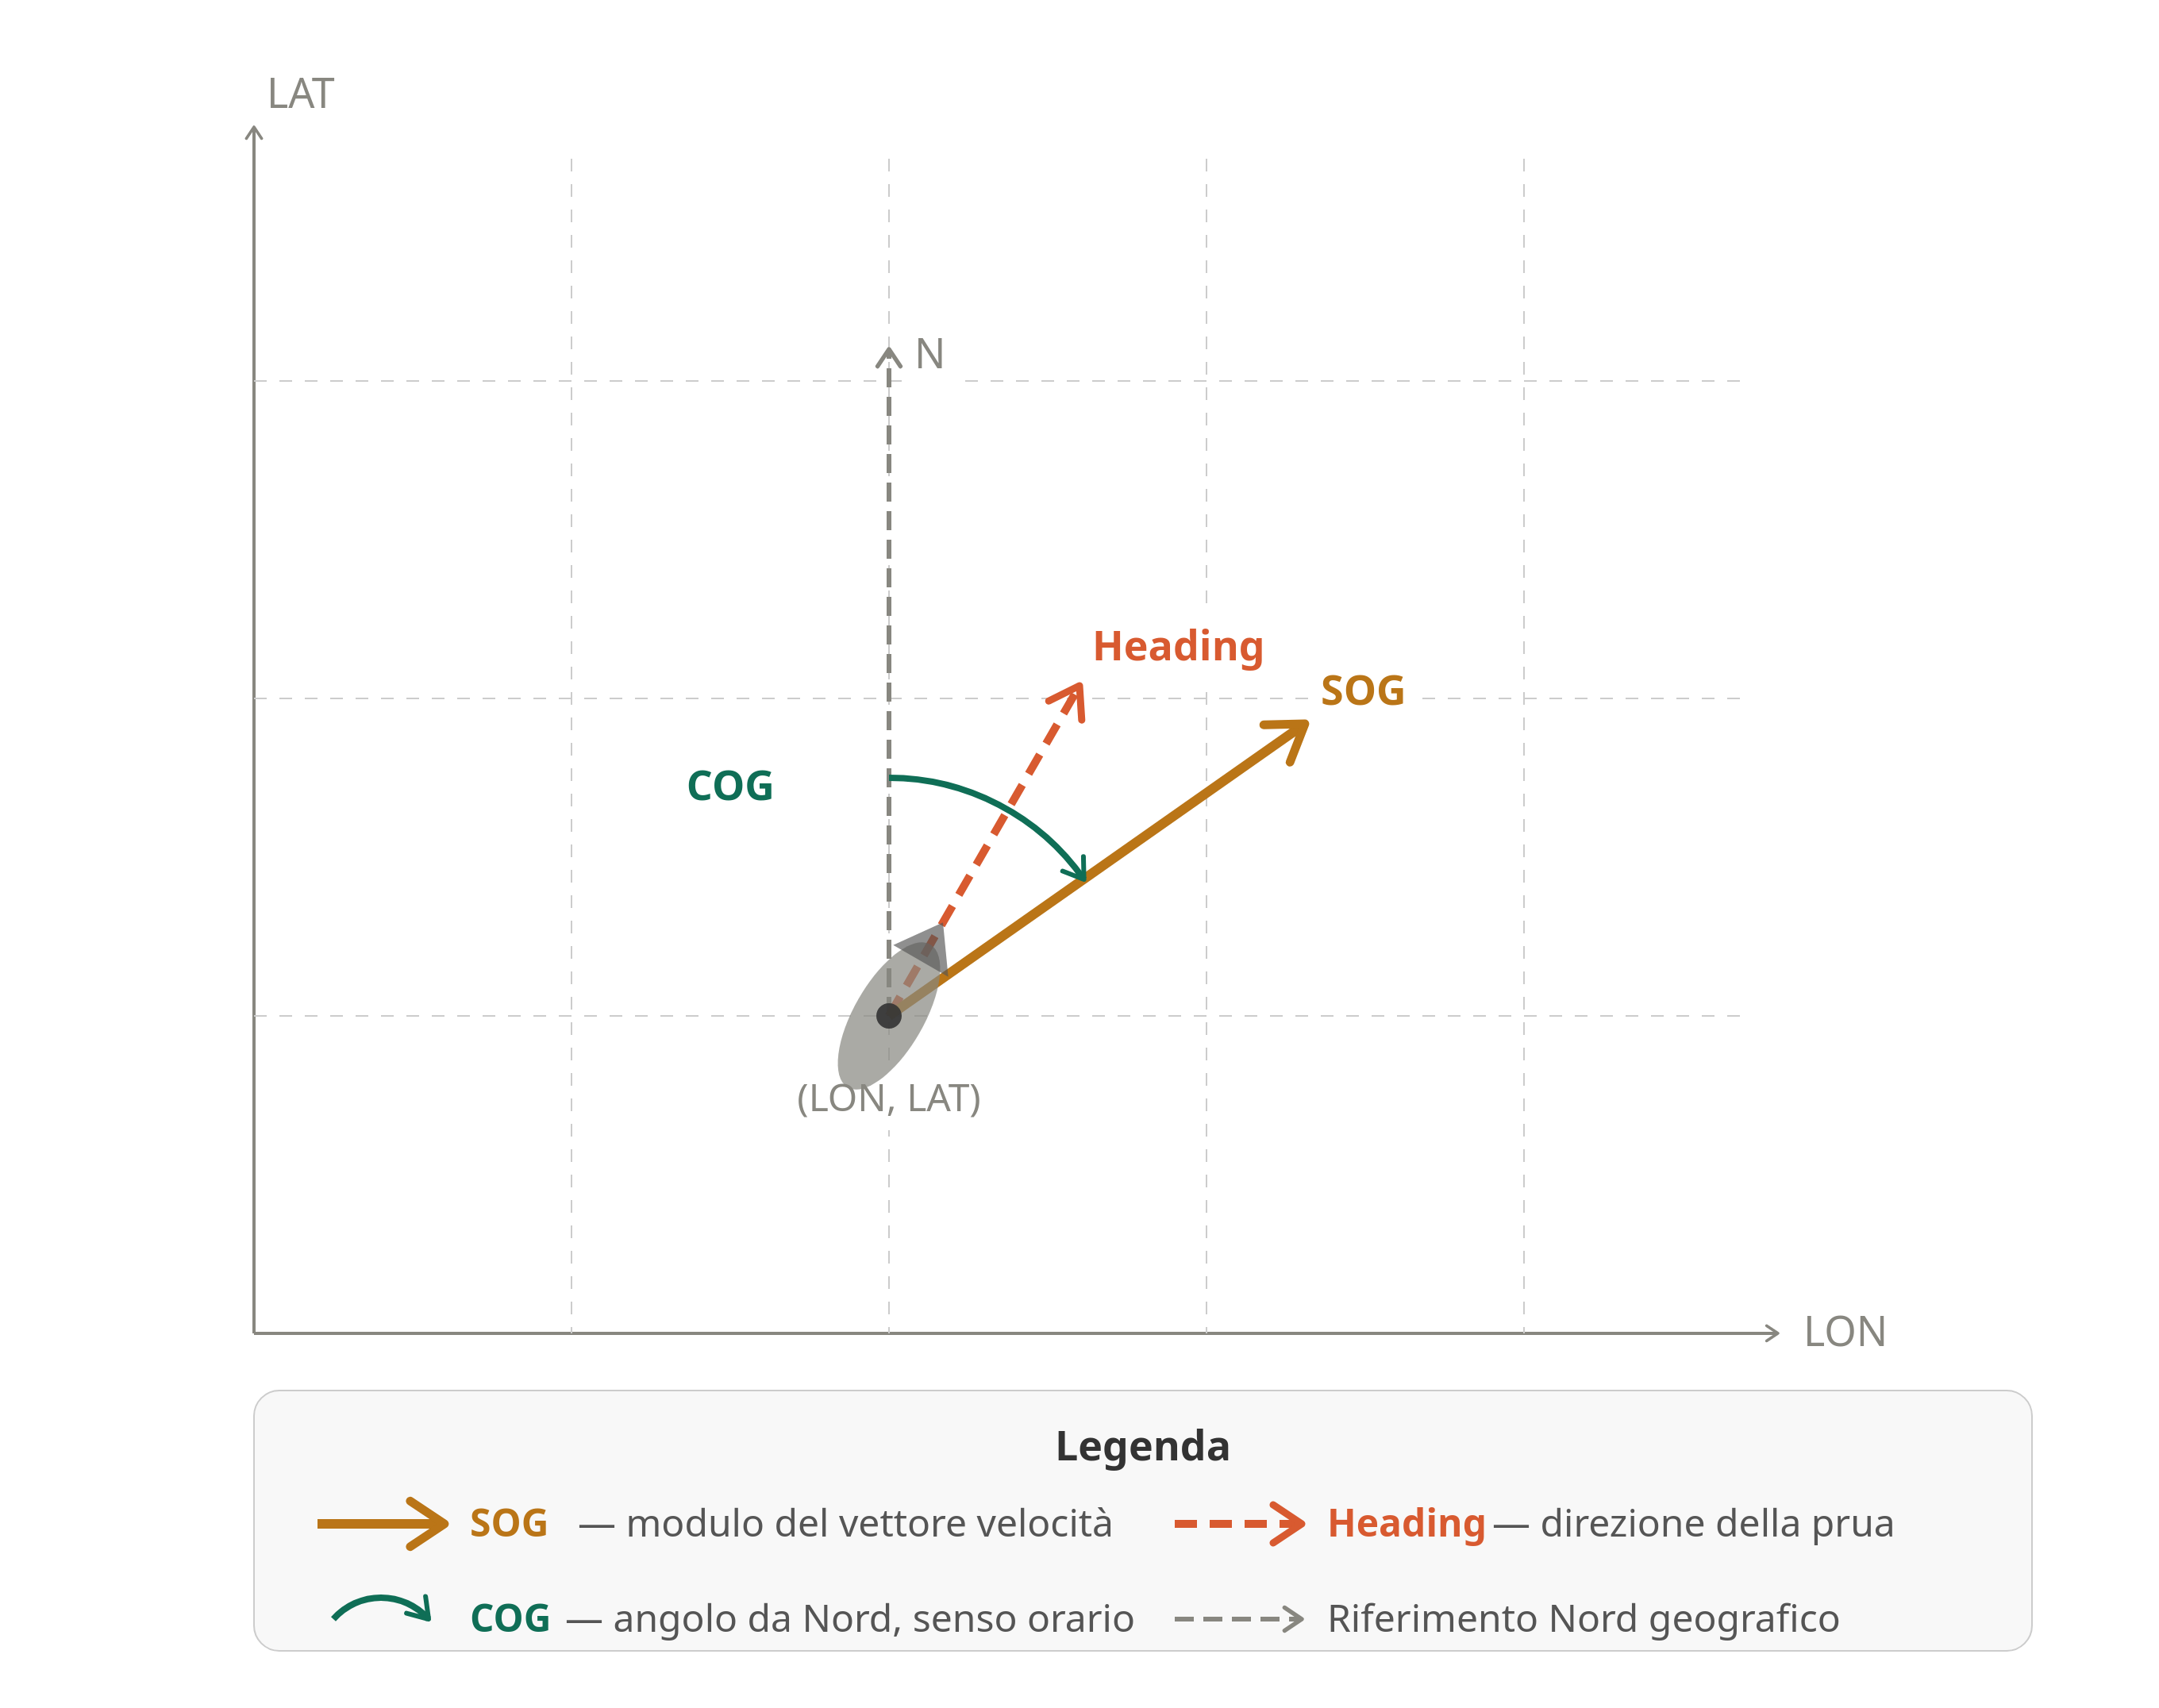
\includegraphics[width=0.75\textwidth]{Methodology/vessel_cog_sog_heading.png}
    \caption{Rappresentazione cartesiana di un record AIS.\@}\label{fig:ais_vessel_diagram}
\end{figure}

\begin{figure}[htbp]
    \centering
    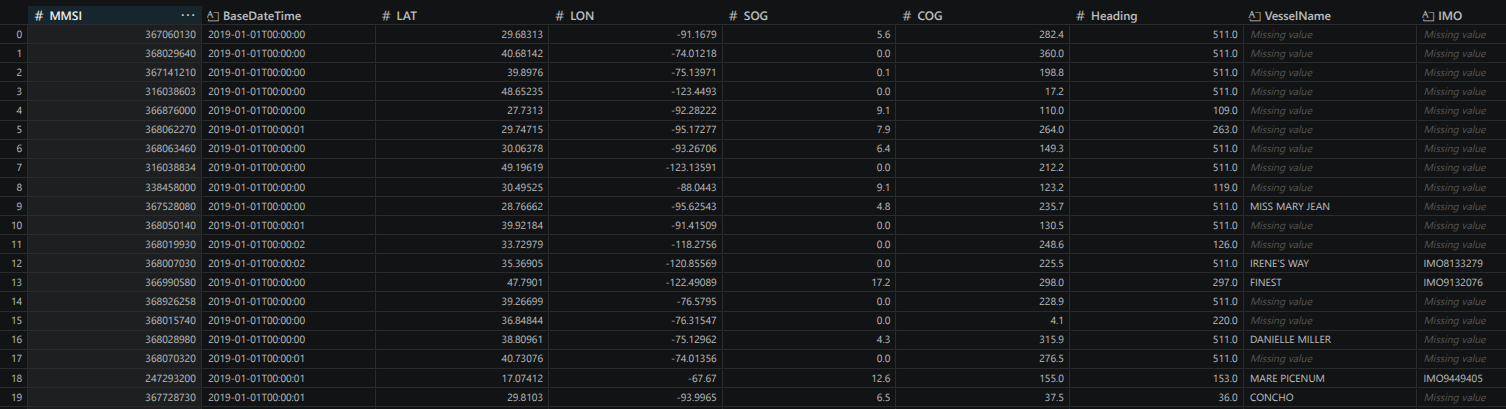
\includegraphics[width=\textwidth]{Methodology/Estratto_dataset.png}
    \caption{Estratto del dataset di partenza.}\label{fig:Estratto_dataset}
\end{figure}

In figura~\ref{fig:Estratto_dataset} è possibile vedere un esempio dei dati contenuti nelle colonne
\texttt{MMSI, BaseDateTime, LAT, LON, SOG, COG, Heading, VesselName, IMO}  

\subsection{Qualità dei dati}\label{ssec:meth_dataset_quality}

Oltre alla struttura, è opportuno considerare la qualità intrinseca dei dati. Un vantaggio rilevante del dataset NOAA
rispetto ad altre fonti pubbliche (in particolare i dati danesi considerati e poi scartati in fase esplorativa) è che
i dati sono già stati filtrati dagli errori più grossolani, rendendo l'uso di tecniche di pulizia aggiuntive meno
critico. È stata tuttavia mantenuta l'assunzione esplicita che le colonne \texttt{MMSI} e \texttt{BaseDateTime} 
siano affidabili e prive di errori, in quanto queste due colonne costituiscono la base di tutte le elaborazioni successive.

% -----------------------------------------------------------------------
\section{Pre-processing dei dati}\label{sec:meth_preprocessing}

L'intera fase di pre-processing, nonchè le successive analisi, sono implementate in Python, utilizzando dei notebook Jupyter.
Le tecnologie utilizzate verranno descritte meglio nella Sezione~\ref{sec:meth_technologies}.

\subsection{Importazione, filtraggio geografico e rimozione dei duplicati}

I file scaricati dalla piattaforma del NOAA sono in formato ``.zip''. Pertanto vengono automaticamente decompressi
e successivamente eliminati dal disco per liberare spazio, mentre i file csv così estratti vengono mantenuti.
Il nome di ogni archivio decompresso viene registrato in un apposito file di log, così da non ripetere l'operazione
nelle esecuzioni successive.
Durante l'importazione, ogni file csv letto viene salvato in memoria sottoforma di \texttt{DataFrame}. In questa fase, 
vengono immediatamente scartati tutti quei messaggi le cui coordinate di latitudine e longitudine ricadono
al di fuori del perimetro citato nella sezione~\ref{sec:meth_dataset}.
Tutti i \texttt{DataFrame} così creati vengono concatenati in un unico \texttt{DataFrame} finale, che viene esportato in un unico file CSV di backup.
Le operazioni di importazione e filtraggio avvengono grazie alla libreria \textbf{Polars}, che è stata scelta per il fatto che (a differenza
di Pandas) supporta il multithreading nativamente. 

In una fase successiva, i record esattamente duplicati (identici in ogni attributo) vengono rimossi, lasciandone solo uno per ogni gruppo duplicato.

Viene poi rimosso un ulteriore sottoinsieme di record: quelli generati da navi, la cui somma di record presenti nel database è inferiore
al 10\% della media calcolata sul totale delle navi presenti. 
Per identificare l'appartenenza di un record ad una nave o meno, è stato utilizzato il valore di \texttt{MMSI}. Come citato in precedenza alla
sezione~\ref{ssec:meth_dataset_quality}, tale attributo si assume corretto e validato dal NOAA in fase di raccolta dei dati.

La soglia usata per rimuovere le navi meno attive è calcolata dinamicamente (e non come valore fisso) in modo
da rendere il codice indipendente dalle dimensioni del dataset che si decide di utilizzare. L'idea dietro la decisione di rimuovere queste navi
 è che, al di sotto di questa soglia, non contribuiscono in maniera significativa al traffico dell'area e la loro presenza potrebbe 
distorcere la fase di clustering.
Prima dell'applicazione di questa soglia il dataset conteneva 602 imbarcazioni distinte (5.460.800 record). In seguito il numero di 
navi distinte è passato a 403 (5.415.168 righe), eliminando 199 vascelli (circa un terzo delle imbarcazioni di partenza) che costituivano 
solo lo 0,84\% dei record totali. 

\subsection{Ottimizzazione della memoria}\label{ssec:meth_memory}

Il dataset pulito viene riletto in Pandas per le elaborazioni successive. Per ridurre il
consumo di memoria (il dataset occupa circa 702 MB nella rappresentazione di default)
i tipi di dato delle colonne vengono convertiti nelle rappresentazioni più compatte
compatibili con i limiti tecnici definiti dalla normativa ITU-R M.1371-6~\cite{itu2026},
che specifica la codifica binaria di ciascun campo del messaggio AIS\@.
La Tabella~\ref{tab:dtype_optimization} riassume le conversioni effettuate con la relativa
giustificazione.

\begin{table}[htbp]
\centering
\caption{Ottimizzazione dei tipi di dato.}\label{tab:dtype_optimization}
\begin{tabular}{lllp{5.5cm}}
\toprule
\textbf{Colonna} & \textbf{Tipo originale} & \textbf{Nuovo tipo} & \textbf{Motivazione} \\
\midrule
\texttt{MMSI} & \texttt{int64} & \texttt{int32} & Codificato su 30 bit; valori fino a 999\,999\,999. Un \texttt{int32} ($\approx 2.1 \times 10^9$) è sufficiente. \\
\texttt{LAT} & \texttt{float64} & \texttt{float64}$^{(a)}$ & Tipo invariato. I valori vengono arrotondati a 4 cifre decimali ($\approx 10$ m di risoluzione) per ridurre il numero di coordinate distinte nelle operazioni di group-by. \\
\texttt{LON} & \texttt{float64} & \texttt{float64}$^{(a)}$ & Stessa giustificazione di \texttt{LAT}. \\
\texttt{SOG} & \texttt{float64} & \texttt{float64} & Tipo invariato. \\
\texttt{COG} & \texttt{float64} & \texttt{float64} & Tipo invariato. \\
\texttt{Heading} & \texttt{float64} & \texttt{float64} & Tipo invariato. \\
\texttt{VesselType} & \texttt{float64} & \texttt{int16}$^{(b)}$ & Formalmente 8 bit (0--255), ma il dataset NOAA presenta valori superiori. I \texttt{NaN} vengono sostituiti con 0. \\
\texttt{Status} & \texttt{float64} & \texttt{int8} & Codificato su 4 bit (valori 0--15). I \texttt{NaN} vengono sostituiti con 99. \\
\texttt{Length} & \texttt{float64} & \texttt{int16} & Valore massimo 511 m. I valori frazionari vengono troncati (errore $< 1$ m). I \texttt{NaN} vengono sostituiti con 0. \\
\texttt{Width} & \texttt{float64} & \texttt{int16} & Stessa giustificazione di \texttt{Length}. \\
\texttt{Draft} & \texttt{float64} & \texttt{float32} & Codificato su 8 bit con risoluzione di 0.1 m, massimo 25.5 m. \\
\texttt{Cargo} & \texttt{float64} & \texttt{int16}$^{(b)}$ & Stessa giustificazione di \texttt{VesselType}. \\
\texttt{TransceiverClass} & \texttt{object} & \texttt{bool} & Assume solo i valori \texttt{A} o \texttt{B}. Rinominato \texttt{IsClassA}. \\
\texttt{BaseDateTime} & \texttt{object} & \texttt{datetime64[s]} & Conversione da object a tipo temporale nativo di Pandas. \\
\midrule
\multicolumn{4}{l}{\footnotesize $^{(a)}$ Tipo invariato; l'unica trasformazione è l'arrotondamento a 4 cifre decimali.} \\
\multicolumn{4}{l}{\footnotesize $^{(b)}$ Scostamento dalla specifica ITU-R M.1371-6, giustificato dai valori presenti nel dataset NOAA.} \\
\bottomrule
\end{tabular}
\end{table}

Le colonne \texttt{VesselName}, \texttt{IMO} e \texttt{CallSign} vengono convertite da
\texttt{object} a\\ \texttt{Pandas.StringDtype}. Questa operazione non produce un risparmio di
memoria significativo, ma garantisce una gestione più corretta dei valori mancanti. Poiché
queste tre colonne non vengono utilizzate nelle elaborazioni successive, non sono incluse
in tabella. Grazie alle conversioni effettuate, il dataset si riduce da circa 702 MB a
circa 465 MB, con un risparmio prossimo al 34\%.

\subsection{Calcolo della velocità media e classificazione degli stati}\label{ssec:meth_status}
 
Una volta completata la fase di importazione e pulizia, l'analisi viene condotta su una nave alla volta utilizzando
il valore di \texttt{MMSI} per distinguerle tra loro.
Per ciascuna nave viene costruito un \texttt{DataFrame} separato, ordinato cronologicamente per \texttt{BaseDateTime} e contenente
tutti messaggi che quell'imbarcazione ha generato nel periodo di analisi all'interno dell'area geografica analizzata.
Per ogni coppia di punti consecutivi appartenenti alla stessa nave viene calcolata la velocità media \texttt{Avg\_Speed},
come rapporto tra la distanza percorsa e l'intervallo di tempo trascorso. La distanza viene calcolata sfruttando la formula
della \emph{Great-Circle Distance}, che tiene conto della curvatura terrestre usando come raggio della Terra il raggio equatoriale definito
dallo standard WGS-84 e pari a 6\,378\,137 m. L'intervallo di tempo tra i due punti
viene individuato facendo la differenza tra i due timestamp e sfruttando l'ordinamento cronologico applicato in precedenza. 
La velocità risultante viene convertita in nodi nautici.
 
Il calcolo viene gestito in modo vettorizzato: ogni traiettoria viene rappresentata come due sequenze di punti sfalsate
di un passo, ottenendo le coppie (punto precedente, punto corrente). Nei casi in cui l'intervallo di tempo
tra due punti consecutivi supera la soglia \texttt{LOST\_TIME\_THRESHOLD\_SECONDS} (impostata a 620 s e corrispondente
a circa 10 volte il periodo tipico di trasmissione di un dispositivo AIS di Classe A), la velocità media del secondo punto appena calcolata
viene scartata e sostituita con il valore di \texttt{SOG}, a condizione che quest'ultimo sia plausibile (inferiore
alla soglia \texttt{ABSURD\_SPEED\_THRESHOLD} di 102 nodi). In caso contrario, la velocità viene ricalcolata
ancora come rapporto distanza/tempo. Al primo punto di ogni traiettoria, per il quale non esiste un punto
precedente, viene assegnato direttamente il valore di \texttt{SOG}. I punti con \texttt{Avg\_Speed} superiore
a 102 nodi (e che non fanno scattare la soglia \texttt{LOST\_TIME\_THRESHOLD\_SECONDS}) vengono eliminati, 
in quanto ritenuti il risultato di errori di posizionamento GPS\@. In totale dal dataset sono stati rimossi 7 record
su 5.415.163 che ricadevano in quest'ultima casistica. 
 
A partire da \texttt{Avg\_Speed}, viene costruita la colonna \texttt{EstimatedStatus}, che classifica ogni punto
in una delle sei categorie seguenti. Le prime quattro riguardano la gestione dei gap temporali e vengono
assegnate durante il calcolo della velocità:
 
\begin{itemize}
    \item \textbf{lost}: record immediatamente precedente un gap temporale superiore a \texttt{LOST\_\allowbreak{}TIME\_\allowbreak{}THRESHOLD\_\allowbreak{}SECONDS}.
          Indica l'ultimo momento in cui la nave era tracciata prima di scomparire temporaneamente dal sistema.
    \item \textbf{return}: primo record successivo al gap citato al punto precedente. Indica il momento in cui la nave torna visibile
          dopo una breve interruzione. I punti \emph{lost} e \emph{return} non entrano nella fase di clustering,
          ma sono utili per la corretta interpretazione delle traiettorie.
    \item \textbf{exit}: record precedente un gap superiore a \texttt{EXIT\_\allowbreak{}TIME\_\allowbreak{}THRESHOLD\_\allowbreak{}HOURS}
          (12 ore). Indica che la nave ha lasciato l'universo di analisi o ha smesso di trasmettere per un periodo
          prolungato.
    \item \textbf{entry}: primo record successivo al gap citato al punto precedente. Indica il rientro della nave 
          nell'universo di analisi dopo un'assenza significativa.
\end{itemize}
 
Gli status \emph{exit} e \emph{entry} vengono assegnati dopo \emph{lost} e \emph{return}, sovrascrivendoli quando
il gap supera la soglia più lunga.
Le restanti due categorie vengono assegnate in una seconda fase, sui punti che non hanno ancora ricevuto uno status:
 
\begin{itemize}
    \item \textbf{stationary}: punti con \texttt{Avg\_Speed} $\leq$ \texttt{SPEED\_THRESHOLD} (0.5 nodi).
    \item \textbf{sailing}: tutti i punti rimanenti, in navigazione ordinaria.
\end{itemize}
 
Al termine, il primo punto di ciascuna traiettoria viene forzato a \emph{entry} e l'ultimo a \emph{exit},
indipendentemente dallo status eventualmente già calcolato. Quando più punti consecutivi risultano tutti \emph{entry} o tutti
\emph{exit} (situazione possibile in presenza di gap ravvicinati) viene conservato solo l'ultimo punto
\emph{entry} della sequenza e il primo punto \emph{exit}, eliminando i rimanenti.

%-----------------------------------------------------------------------------------------------------------
\section{Implementazione del framework TREAD e differenze rispetto all'originale}\label{sec:meth_algorithm}

\subsection{Architettura generale}

Il framework TREAD di Pallotta et al.~\cite{pallotta} si articola in due macro fasi: \emph{Knowledge Discovery} e \emph{Knowledge Exploitation}.
Nella prima fase, il flusso di messaggi AIS viene elaborato per costruire un modello statistico del traffico normale, articolato in tre classi
di oggetti: vessel objects ($Vs$), waypoint objects ($WPS$) e route objects ($Rs$).
Nella seconda fase, le rotte apprese vengono utilizzate per classificare nuove traiettorie e individuare comportamenti anomali.

La presente implementazione riproduce questa struttura a due fasi. Tuttavia, il processo non è incrementale in senso stretto:
anzichè aggiornare il modello messaggio per messaggio come nell'algoritmo originale, l'intero dataset viene caricato in memoria
e processato in batch. Questa scelta è stata motivata dai vincoli hardware descritti nella sezione~\ref{sec:meth_limits}.


\subsection{Identificazione dei waypoint: DBSCAN e H-DBSCAN}\label{ssec:meth_clustering}

Il passo centrale della fase di Knowledge Discovery è l'identificazione dei waypoint. In questo
contesto, un waypoint viene definito come un'area geografica appartenente all'universo di analisi in cui le navi:
\begin{itemize}
    \item iniziano a manifestare la propria presenza nell'universo di analisi (entry);
    \item cessano di manifestare la propria presenza nell'universo di analisi (exit);
    \item rallentano significativamente, con velocità media inferiore alla soglia
          \texttt{SPEED\_\allowbreak{}THRESHOLD} (0.5 nodi), al di sotto della quale la nave è ritenuta
          sostanzialmente stazionaria.
\end{itemize}
A differenza di quanto avviene su terra, in mare è molto difficile per una nave
rimanere completamente ferma per via di correnti, vento e onde che spesso causano qualche tipo di movimento. 
Per questo motivo, anziché cercare punti di velocità nulla, si è deciso di introdurre una soglia
(\texttt{SPEED\_THRESHOLD}) sotto la quale un'imbarcazione è considerata stazionaria. 
I waypoint non hanno dimensione fissa: ciascuno occupa una porzione dello spazio geografico 
determinata da come si distribuiscono e da quanti sono i punti che lo compongono. Nella pratica, la maggior parte di essi 
tende ad occupare un'area molto ridotta rispetto all'universo di analisi.
Nell'algoritmo originale l'identificazione dei waypoint viene effettuata tramite un approccio basato su DBSCAN.\
La presente implementazione applica prima DBSCAN e poi H-DBSCAN come variante
migliorativa (\emph{Hierarchical DBSCAN}).

\subsubsection{Preparazione degli input per il clustering}
 
L'input fornito agli algoritmi di clustering è costituito da tutti i punti classificati come 
\emph{stationary}, \emph{entry} o \emph{exit}, che rappresentano circa il 69,6\% del dataset totale.

Per ridurre la dimensione dell'input e superare le limitazioni di memoria dell'implementazione scikit-learn di DBSCAN, 
il cui costo di memoria è $O(n^2)$, i punti vengono aggregati tramite un'operazione di \emph{group-by} sulle sole coordinate GPS, 
contando quante volte ogni coppia (\texttt{LAT}, \texttt{LON}) compare nel dataset. Questa operazione è il motivo per cui si è deciso
di arrotondare da 5 a 4 cifre decimali i valori di latitudine e longitudine (vedi Tabella~\ref{tab:dtype_optimization}). 
Così facendo si riduce il numero di coppie distinte in input all'algoritmo di clustering e allo stesso tempo la perdita di precisione
è considerata trascurabile. Infatti, con 5 cifre decimali la risoluzione massima è attorno ad 1 metro; con 4 cifre decimali la risoluzione 
passa a circa 10 metri.
Le somme risultanti dall'operazione di \emph{group-by} vengono utilizzate come \emph{pesi} da associare a ciascuna coordinata, allo scopo
di rappresentare la frequenza con cui ogni posizione è stata visitata.
Tuttavia si è notato che esistono diversi dispositivi statici (es: boe, stazioni costiere) che, dotati di transponder AIS, restano stazionari
in un punto e continuano periodicamente a trasmettere, riempendo il database. 
Per attenuare lo sbilanciamento tra queste coordinate che all'apparenza sembrano molto visitate e le altre coordinate, 
i pesi vengono normalizzati applicando il logaritmo base 2 e approssimando il risultato all'intero piu vicino; 
infine le coordinate con peso zero dopo la trasformazione logaritmica vengono riportate artificialmente a 1.
La tabella risultante usata come input per l'applicazione dell'algoritmo di DBSCAN ha circa 52.000 righe, mentre il numero di 
punti stazionari processati è pari a circa 3.770.000 righe.


\subsubsection{DBSCAN}
 
L'algoritmo DBSCAN viene eseguito con i parametri $\varepsilon = 0.075$ e $N_{\min} = 10$, scelti empiricamente 
in modo da produrre cluster geograficamente coerenti con i porti e i punti di passaggio dell'arcipelago delle Hawaii. 
Questo passo riproduce l'approccio di Pallotta et al.\ ed è incluso come riferimento per il confronto con la variante H-DBSCAN\@.

\subsubsection{H-DBSCAN}
 
Il motivo principale per introdurre H-DBSCAN è la sua capacità di identificare cluster di densità variabile, cosa che DBSCAN non 
riesce a gestire bene. %~\cite{schubert2017}. 
Il traffico nelle Hawaii presenta una densità fortemente eterogenea: i porti principali come Honolulu hanno concentrazioni 
di punti molto più elevate rispetto a zone di passaggio o porti minori. 
In questo contesto, i parametri fissi di DBSCAN tendono a sovra-segmentare le aree sparse o a fondere artificialmente cluster distinti 
nelle aree dense.
 
Poiché la libreria \texttt{hdbscan}\footnote{Libreria esterna \texttt{hdbscan} (\url{https://github.com/scikit-learn-contrib/hdbscan}), 
distinta dall'implementazione inclusa in scikit-learn.} non consente di associare i pesi ad ogni punto ma li considera tutti equiponderati, 
la tabella aggregata viene espansa: ogni coordinata viene replicata un numero di volte pari al suo peso calcolato in precedenza applicando il logaritmo. 
La tabella espansa conta circa 97.000 righe, ossia poco meno del doppio della tabella utilizzata come input per l'algoritmo DBSCAN\@. 
Infine, H-DBSCAN viene eseguito con i parametri $\text{min\_cluster\_size} = 30$, $\text{max\_cluster\_size} = 10\,000$ 
e $\text{cluster\_selection\_epsilon} = 0.01$.

\subsection{Costruzione dei waypoint e identificazione delle rotte}\label{ssec:meth_routes}
 
Una volta determinati i cluster tramite H-DBSCAN, per ciascun cluster viene calcolato il \emph{convex hull} (inviluppo convesso) 
tramite \texttt{scipy.spatial.ConvexHull}. L'inviluppo convesso di ogni cluster definisce il perimetro del waypoint corrispondente, 
rappresentato come un poligono tramite la libreria Shapely.
 
Per ogni punto del dataset viene quindi verificato se esso ricade all'interno o sul bordo
di uno dei poligoni waypoint, informazione salvata nella colonna \texttt{IsInWP}.
Il bordo viene incluso perché i vertici dell'inviluppo convesso sono essi stessi punti del
dataset: escludendoli, tali punti risulterebbero esterni al
waypoint che contribuiscono a definire.
Poiché gli inviluppi convessi di cluster diversi possono sovrapporsi, un punto può ricadere
in più di un waypoint; in tal caso viene assegnato a quello con indice minore.
Per valutare l'impatto di questa scelta, viene inoltre calcolato il numero di punti che
ricadono in più di un waypoint.
Un waypoint è considerato \emph{significativo} per un dato punto se quest'ultimo soddisfa almeno una delle condizioni seguenti: 
\texttt{Avg\_Speed} $\leq$ \texttt{SPEED\_THRESHOLD}, oppure il suo \texttt{EstimatedStatus} è \emph{entry} o \emph{exit}.


L'assegnazione delle rotte avviene una nave alla volta, all'interno di ogni coppia
(\emph{entry}, \emph{exit}) identificata nel dataset. A ogni punto viene assegnata
un'etichetta secondo la seguente logica:
\begin{itemize}
    \item se il punto si trova all'interno di un waypoint significativo, l'etichetta
          corrisponde al nome di quel waypoint;
    \item se il punto si trova in navigazione tra due waypoint, l'etichetta assume il
          formato \texttt{WP\_X --- WP\_Y}, dove \texttt{WP\_X} e \texttt{WP\_Y} sono
          rispettivamente il waypoint di provenienza e quello di destinazione; nei casi
          in cui uno o entrambi non siano identificabili, viene utilizzato il
          segnaposto \texttt{<NA>}.
\end{itemize}

Con queste ultime operazioni, termina la fase di Knowledge Discovery: ogni punto
del dataset ha associata un'etichetta di rotta secondo i criteri appena descritti, e il
modello di traffico appreso è pronto per essere utilizzato nella fase di Knowledge
Exploitation.

% -----------------------------------------------------------------------
\section{Anomaly detection}\label{sec:meth_anomaly}
 
Prima di descrivere la fase di anomaly detection, è opportuno distinguere due concetti
fondamentali. Una \textbf{rotta} è un'entità astratta che modella il fatto che almeno una volta una 
nave ha viaggiato dal waypoint di partenza a quello di arrivo (e non il viceversa).
Ipotizzando di modellare i waypoint come nodi di un grafo orientato, una rotta sarebbe uno degli archi.
Un \textbf{trip} indica invece il singolo viaggio compiuto da una specifica nave lungo una rotta. 
A ogni rotta possono quindi essere associati più trip, tanti quante sono le navi che l'hanno percorsa nel
periodo analizzato.

La fase di anomaly detection segue le equazioni del framework TREAD originale~\cite{pallotta}.
 L'analisi si concentra su una singola rotta selezionata (una delle più trafficate tra quelle estratte nella fase precedente) 
 e utilizza i trip associati a tale rotta come unità di analisi.
 
\subsection{Decomposizione della velocità e preparazione delle feature}
 
Per ogni punto del dataset vengono calcolate le componenti cartesiane della velocità $V_x$
e $V_y$ a partire da \texttt{SOG} e \texttt{COG}. Il COG, espresso in gradi rispetto al
nord geografico (angolo \emph{bearing}), viene convertito in angolo aritmetico standard
tramite la formula $\theta = (450 - \text{COG}) \mod 360$, e poi in radianti. Le componenti
risultanti sono:
\[
V_x = \text{SOG} \cdot \cos(\theta), \qquad V_y = \text{SOG} \cdot \sin(\theta)
\]
Pallotta et al.\ \cite{pallotta} propongono un approccio alternativo per il calcolo
delle stesse componenti, basato sulla funzione arcotangente e sul teorema di Pitagora.
Questo approccio presenta alcune criticità. In primo luogo, la funzione arcotangente è
definita a meno di un'ambiguità di segno: per ricavare il quadrante corretto della
direzione è necessario gestire esplicitamente i casi in cui $V_x$ e $V_y$ assumono segno
negativo, introducendo logica condizionale aggiuntiva. In secondo luogo, l'uso combinato
di arcotangente e radice quadrata è computazionalmente più oneroso rispetto al calcolo
diretto tramite seno e coseno. Infine, l'approccio inverso introduce potenziali errori
numerici nelle situazioni limite, come velocità molto prossime a zero, in cui il rapporto
tra le componenti diventa instabile. Per questi motivi, nella presente implementazione si
è preferito calcolare $V_x$ e $V_y$ direttamente tramite seno e coseno dell'angolo
$\theta$, ottenendo un codice più semplice ed efficiente.


\subsection{Stima della densità tramite Kernel Density Estimation}
 
Per modellare il comportamento normale di una rotta, viene stimata la distribuzione spaziale 
dei punti tramite \emph{Kernel Density Estimation} (KDE) bivariata sui valori di latitudine e Longitudine 
(\texttt{LON}, \texttt{LAT}), usando la funzione \texttt{scipy.stats.gaussian\_kde}. 
Viene inoltre calcolata una seconda KDE, pesata per la magnitudine della velocità (\texttt{SOG}), 
che cattura le zone dove le navi transitano tipicamente a velocità elevate. 
Il prodotto punto per punto delle due KDE (equazione~8 di~\cite{pallotta}) fornisce per ogni punto del dataset 
un valore di densità $p_i$ che combina informazione spaziale e cinematica.


\subsection{Classificazione dei trip per lunghezza}
 
I trip associati alla rotta selezionata vengono ordinati per lunghezza (numero di punti) in ordine crescente. 
Questo ordinamento riflette l'assunzione secondo cui i trip più corti sono maggiormente rappresentativi del 
comportamento normale, mentre i trip più lunghi o devianti hanno una maggiore probabilità di essere anomali; 
tale assunzione guida l'interpretazione del ranking di anomalia descritto nella sezione successiva, ma 
l'intero insieme dei trip disponibili viene utilizzato sia per la stima dei parametri del modello sia per 
il calcolo dello score di anomalia.
 
\subsection{Calcolo della probabilità di transizione e anomaly scoring}
 
Il modello di anomaly detection si basa sulla probabilità di transizione tra stati successivi 
di una traiettoria, modellata tramite una distribuzione di Weibull, seguendo l'equazione~14 di~\cite{pallotta}:
\[
p(\Delta p \mid \Delta t) = \exp\!\left[-{\left(\frac{\Delta p}{m \cdot \Delta t}\right)}^{\beta}\right]
\]
dove $\Delta t$ è l'intervallo di tempo e $\Delta p$ è la distanza tra la posizione effettiva
e quella predetta tramite il Track Predictor (algoritmo~4 di~\cite{pallotta}).
Quest'ultimo stima la posizione futura ipotizzando che la nave proceda con la stessa direzione
e la stessa velocità dell'ultima osservazione. Lo spostamento viene calcolato a partire dalle
componenti della velocità $v_x = \mathrm{SOG}\cos\theta$ (verso est) e $v_y = \mathrm{SOG}\sin\theta$ (verso nord),
dove $\theta = (450^\circ - \mathrm{COG}) \bmod 360^\circ$ è la rotta convertita in angolo aritmetico.
Lo spostamento, espresso in miglia nautiche, viene convertito in gradi considerando che un miglio
nautico corrisponde a $1/60$ di grado di latitudine, mentre in longitudine il valore va ulteriormente
diviso per $\cos(\mathrm{lat})$.
La distanza $\Delta p$, espressa in metri, è infine calcolata in maniera analoga a quanto descritto
nella Sezione~\ref{ssec:meth_status}.
I parametri $m$ e $\beta$ del modello sono stimati sull'intero insieme di trip disponibili.
I parametri vengono stimati calcolando, per un insieme di lag temporali adattativi 
(da un minimo di 30 s a un massimo di un quinto della durata mediana dei trip), 
le distribuzioni delle distanze $\Delta p$ e fittando su ciascuna una distribuzione di Weibull 
tramite \texttt{scipy.stats.weibull\_min}. 
Il parametro di scala $\alpha_k = m \cdot \Delta t$ viene stimato tramite regressione lineare 
sull'insieme dei valori ottenuti ai diversi lag; il parametro di forma $\beta$ è preso come media dei valori stimati.
 
Ad ogni trip viene infine assegnato un punteggio di anomalia come log-somma normalizzata 
delle probabilità di transizione lungo la traiettoria (equazione~9 di~\cite{pallotta}), 
combinata con la log-probabilità di osservazione derivata dalla KDE (equazione~6) e con la probabilità a priori della rotta (equazione~4).
Quest'ultima è stimata, come in~\cite{pallotta}, come il rapporto tra il numero di navi distinte
che percorrono la rotta e il numero totale di navi considerate. Poiché l'analisi è condotta su
una sola rotta, la probabilità a priori risulta pari a 1 per tutti i trip e non influisce sul ranking;
il termine viene comunque mantenuto nell'implementazione per consentire l'estensione dell'analisi a più rotte.
I trip con punteggio più basso sono classificati come potenzialmente anomali.



\section{Tecnologie utilizzate}\label{sec:meth_technologies}

L'intera pipeline è implementata in \textbf{Python 3}, organizzata in file Jupyter Notebook separati. 
I parametri di configurazione sono centralizzati in un unico file ``.py'' a cui hanno accesso tutti i Notebook Jupyter.

Le librerie principali utilizzate sono:

\begin{itemize}
    \item \textbf{Polars}: per sfruttare il multithreading durante l'importazione dei file CSV giornalieri e il filtraggio geografico iniziale;
    \item \textbf{Pandas}: per la manipolazione del dataset nelle fasi successive all'importazione;
    \item \textbf{NumPy}: per i calcoli vettoriali e le operazioni sulle serie temporali;
    \item \textbf{scikit-learn}: per l'implementazione di DBSCAN\@;
    \item \textbf{hdbscan}: libreria per H-DBSCAN, scelta per le sue prestazioni superiori rispetto all'implementazione scikit-learn nella gestione di cluster di densità variabile;
    \item \textbf{SciPy}: per il calcolo dei convex hull, la Kernel Density Estimation e il fitting della distribuzione di Weibull;
    \item \textbf{Shapely}: per le operazioni geometriche sui poligoni waypoint;
    \item \textbf{GeoPandas}: per la visualizzazione rapida dei poligoni waypoint per verifiche qualitative;
    \item \textbf{Plotly}: per la visualizzazione interattiva dei risultati su mappa geografica.
\end{itemize}

La scelta di Python è motivata dalla disponibilità di un ecosistema maturo per l'analisi di dati anche geospaziali e la sua
relativa facilità di utilizzo.



\section{Limiti della metodologia}\label{sec:meth_limits}

La metodologia presentata in questo capitolo presenta alcuni limiti che è opportuno
dichiarare esplicitamente. Un primo limite riguarda la copertura geografica: il dataset
del NOAA è limitato alle aree costiere statunitensi, e la tesi si concentra sulle Hawaii,
un arcipelago con un traffico relativamente contenuto rispetto ad aree come lo Stretto di
Gibilterra o l'Adriatico settentrionale studiate nell'articolo originale di Pallotta et
al.~\cite{pallotta}. I risultati ottenuti potrebbero quindi non generalizzarsi ad aree
con densità di traffico diverse.

Un secondo limite è di natura computazionale: l'implementazione scikit-learn di DBSCAN ha
un costo in memoria $O(n^2)$ rispetto al numero di punti in input (si veda il
Paragrafo~\ref{ssec:meth_clustering} per i dettagli). La RAM disponibile sulla macchina
utilizzata non era sufficiente per eseguire l'algoritmo direttamente sui punti grezzi del
dataset, rendendo necessaria una fase di pre-aggregazione per coordinate GPS e, per
H-DBSCAN, un'ulteriore espansione della tabella dei pesi. Questo livello aggiuntivo di
elaborazione non comporta una perdita di informazione sul dataset nel suo complesso ma
rappresenta comunque un vincolo imposto dall'hardware, che con risorse maggiori non
sarebbe stato necessario.

Un ulteriore limite, intrinseco alla tecnologia AIS stessa e già discusso nel
Capitolo~\ref{chap:literature}, riguarda la natura dei dati alla fonte. Il sistema AIS
traccia esclusivamente le imbarcazioni che montano e utilizzano attivamente il
transponder: l'obbligo di installazione, imposto dalla convenzione SOLAS, si applica
infatti solo alle navi con stazza lorda superiore a una certa soglia e alle navi passeggeri~\cite{imo2004}. 
Il naviglio minore (imbarcazioni da diporto, pescherecci di piccole dimensioni, mezzi non commerciali) 
non è quindi soggetto a tale obbligo e risulta nella maggior parte dei casi del tutto assente dal
dataset. Ne consegue che il modello di traffico appreso descrive esclusivamente il
comportamento delle imbarcazioni di maggiori dimensioni, mentre eventuali pattern di
traffico generati dal naviglio minore restano completamente invisibili.
A questo si aggiungono i limiti di qualità del dato già discussi nel
Capitolo~\ref{chap:literature}, quali le lacune di copertura dei ricevitori terrestri e
la possibilità di manipolazione dei messaggi tramite spoofing o spegnimento volontario
del transponder~\cite{riassuntone}, fattori che, seppur non specificamente analizzati in
questa tesi, contribuiscono al divario tra il traffico realmente presente nell'area e
quello effettivamente osservabile tramite AIS\@.


\section{Sintesi e anticipazione dei risultati}\label{sec:meth_summary}

Il capitolo ha descritto la metodologia adottata per replicare, adattare e estendere il framework TREAD 
di Pallotta et al.\ su dati AIS reali relativi alle Hawaii. 
La pipeline comprende una fase di pre-processing (importazione, pulizia e ottimizzazione, calcolo della velocità media 
e classificazione degli stati), la fase di Knowledge Discovery con il doppio utilizzo di DBSCAN e H-DBSCAN 
per l'identificazione dei waypoint e la successiva assegnazione delle rotte, 
e infine una fase di anomaly detection basata su KDE e distribuzione di Weibull.

Le principali differenze rispetto all'algoritmo originale sono: l'adozione di H-DBSCAN al posto di DBSCAN incrementale, 
motivata dalla necessità di gestire cluster a densità variabile; 
l'approccio batch in luogo di quello incrementale, imposto dai vincoli hardware; 
l'introduzione della normalizzazione per lunghezza del trip nel calcolo del punteggio di anomalia, non presente nell'originale.

Il Capitolo~\ref{chap:results} presenterà i risultati ottenuti: i waypoint identificati, 
le rotte estratte, i parametri del modello Weibull stimati e il ranking di anomalia dei trip sulla rotta selezionata.

% Results
% sections/results.tex
\chapter{Risultati}\label{chap:results}
 
Questo capitolo presenta i risultati ottenuti applicando la pipeline descritta nel
Capitolo~\ref{chap:methodology} al dataset AIS delle Hawaii.
I risultati sono organizzati in quattro sezioni: la prima descrive il dataset nelle
sue dimensioni finali dopo il pre-processing; la seconda mostra i risultati qualitativi
prodotti dalla fase di Knowledge Discovery; la terza riporta i risultati quantitativi
della fase di anomaly detection; la quarta ne discute l'interpretazione e le implicazioni.
 
% ─────────────────────────────────────────────
\section{Dataset}\label{sec:res_dataset}
 
Il dataset utilizzato comprende i messaggi AIS ricevuti dal NOAA nel primo trimestre
del 2019 (gennaio-marzo inclusi), filtrati sull'area geografica delle Hawaii tramite
la bounding box descritta nella Sezione~\ref{sec:meth_dataset}.
 
\subsection{Dimensioni e composizione}
 
I dati grezzi, dopo il filtraggio geografico, ammontano a 5.462.415 record. A seguito
della rimozione dei duplicati esatti il dataset si riduce a 5.460.800 record, generati
da 602 imbarcazioni distinte (in media 9.071 record per nave, con un minimo di 1 e un
massimo di 82.554).
 
L'applicazione della soglia dinamica sull'attività delle imbarcazioni
(Sezione~\ref{sec:meth_preprocessing}), pari al 10\% del numero medio di record per
nave e quindi a 907 record, ha eliminato 199 imbarcazioni, corrispondenti allo 0,84\%
dei record totali. Il dataset risultante conta 5.415.168 record relativi a 403
imbarcazioni, sulle quali si osservano le seguenti statistiche sul numero di record per
nave: media di 13.437 record, deviazione standard di 16.309, con un massimo di 82.554 e
un minimo di 921 record per singola imbarcazione.
 
Dopo la fase di ottimizzazione della memoria, il dataset è passato da circa 702~MB a
circa 465~MB, con un risparmio prossimo al 34\%.
 
\subsection{Classificazione degli stati e punti stazionari}
 
Nella fase di classificazione degli stati di navigazione, 7 record sono stati rimossi
in quanto associati a velocità istantanee non plausibili (superiori a 102 nodi),
portando il dataset a 5.415.156 record complessivi. Di questi, 3.766.844 punti sono
stati classificati come stazionari (comprendendo gli stati \emph{stationary},
\emph{entry} ed \emph{exit}), e costituiscono l'insieme di partenza per la fase di
Knowledge Discovery. L'aggregazione di questi punti per coordinate ha prodotto
51.801 coppie di coordinate distinte.
 
\subsection{Waypoint e rotte estratte}
 
Il clustering H-DBSCAN applicato ai punti stazionari aggregati ha identificato
144 waypoint distinti (da \texttt{WP\_0} a \texttt{WP\_143}).
I punti che ricadono in più di un waypoint, a causa della sovrapposizione degli inviluppi
convessi, sono 7.298, pari allo 0,135\% del dataset: l'effetto della regola di assegnazione
descritta nella Sezione~\ref{ssec:meth_routes} è quindi trascurabile. A partire da questi waypoint,
sono state estratte in tutto 910 rotte distinte e 35.731 trip.
 
Per la fase di anomaly detection è stata selezionata la rotta \texttt{WP\_135 - WP\_118},
una delle più trafficate tra quelle estratte, percorsa da 40 imbarcazioni distinte
per un totale di 184 trip. La lunghezza dei trip (in numero di punti) presenta una
media di 110,0, una mediana di 95,5, un minimo di 41 e un massimo di 524 punti.
 
% ─────────────────────────────────────────────
\section{Risultati qualitativi}\label{sec:res_qualitative}
 
Questa sezione mostra gli output visivi prodotti dalla fase di Knowledge Discovery,
con l'obiettivo di verificare che i waypoint e le rotte estratte corrispondano a
strutture geograficamente coerenti con il traffico marittimo dell'arcipelago delle
Hawaii.
 
\subsection{Waypoint identificati}
 
Le Figure~\ref{fig:res_dbscan} e~\ref{fig:res_hdbscan} mostrano i cluster di punti
stazionari ottenuti rispettivamente con DBSCAN ($\varepsilon = 0.075$, $N_{\min} = 10$)
e con H-DBSCAN ($\text{min\_cluster\_size} = 30$, $\text{max\_cluster\_size} = 10\,000$),
con i parametri descritti nella Sezione~\ref{ssec:meth_clustering}. In entrambe le figure
i punti in blu sono quelli assegnati a un cluster, i punti bianchi sono quelli classificati
come rumore, e il contorno nero di ogni cluster è il relativo \emph{convex hull}, che
definisce l'area del waypoint. Il riquadro rosso è la bounding box dell'area di studio.
La scala di colore indica il peso di ciascuna coordinata aggregata, pari al logaritmo in
base 2 del numero di messaggi AIS che vi ricadono, arrotondato all'intero più vicino
(Sezione~\ref{ssec:meth_clustering}); si tratta quindi di una grandezza adimensionale.

\begin{figure}[htbp]
    \centering
    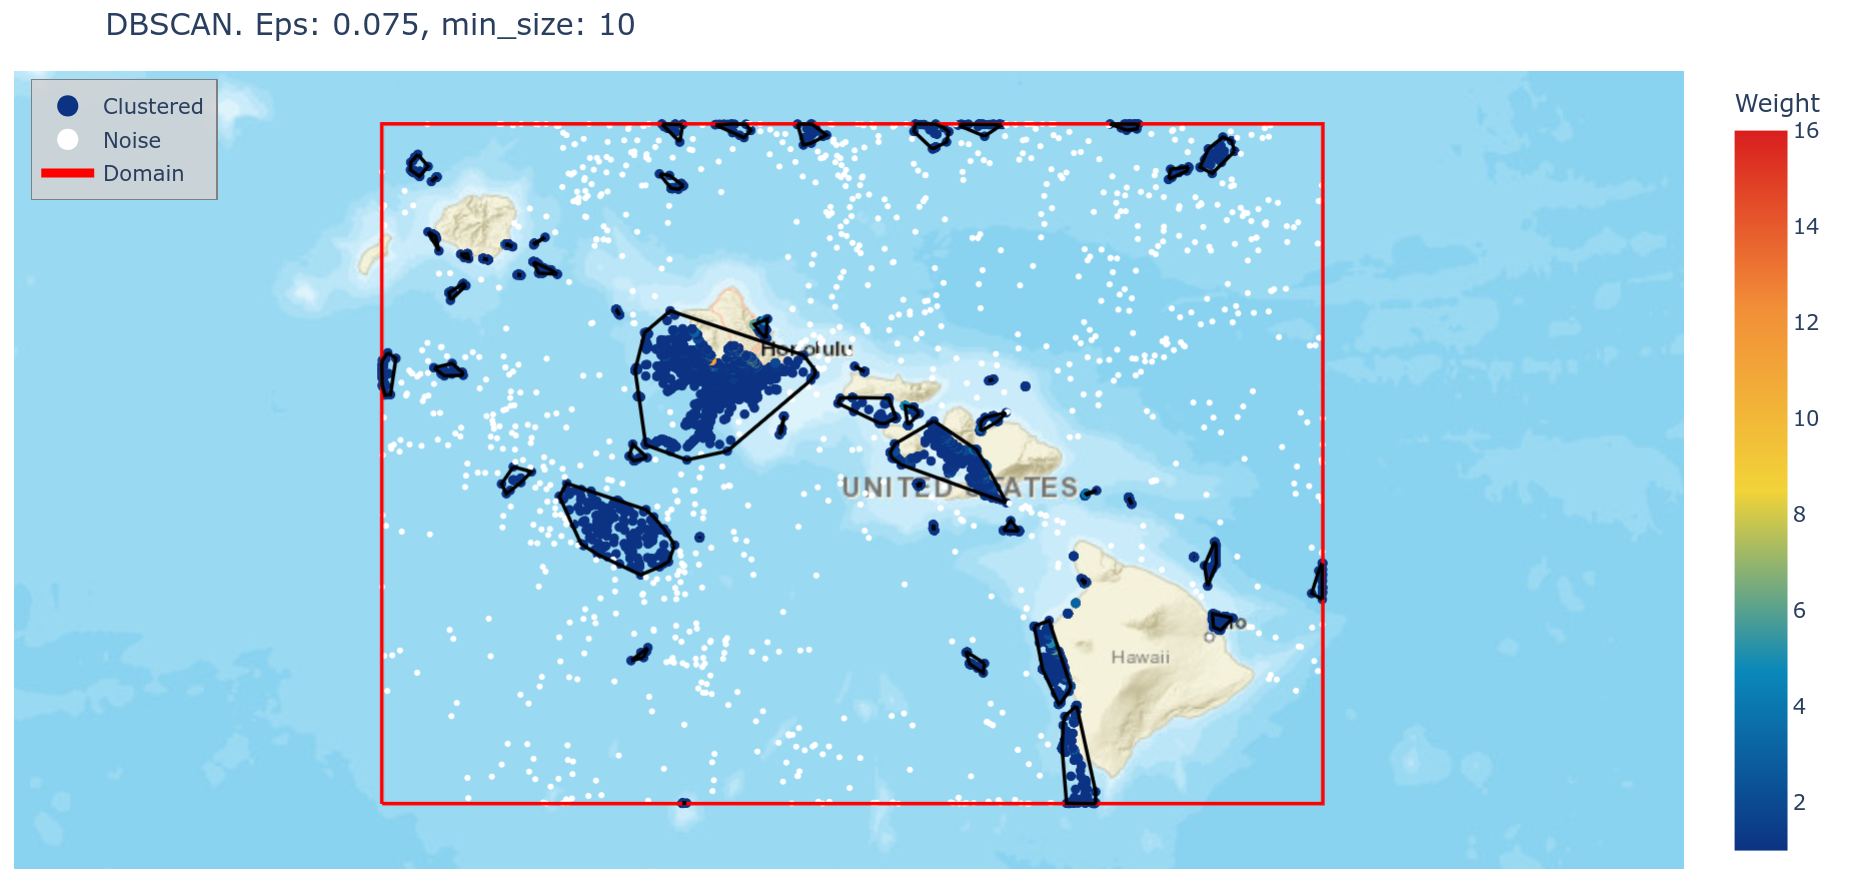
\includegraphics[width=\textwidth]{Results/DBSCAN.png}
    \caption{Waypoint identificati con DBSCAN ($\varepsilon = 0.075$, $N_{\min} = 10$).}\label{fig:res_dbscan}
\end{figure}

\begin{figure}[htbp]
    \centering
    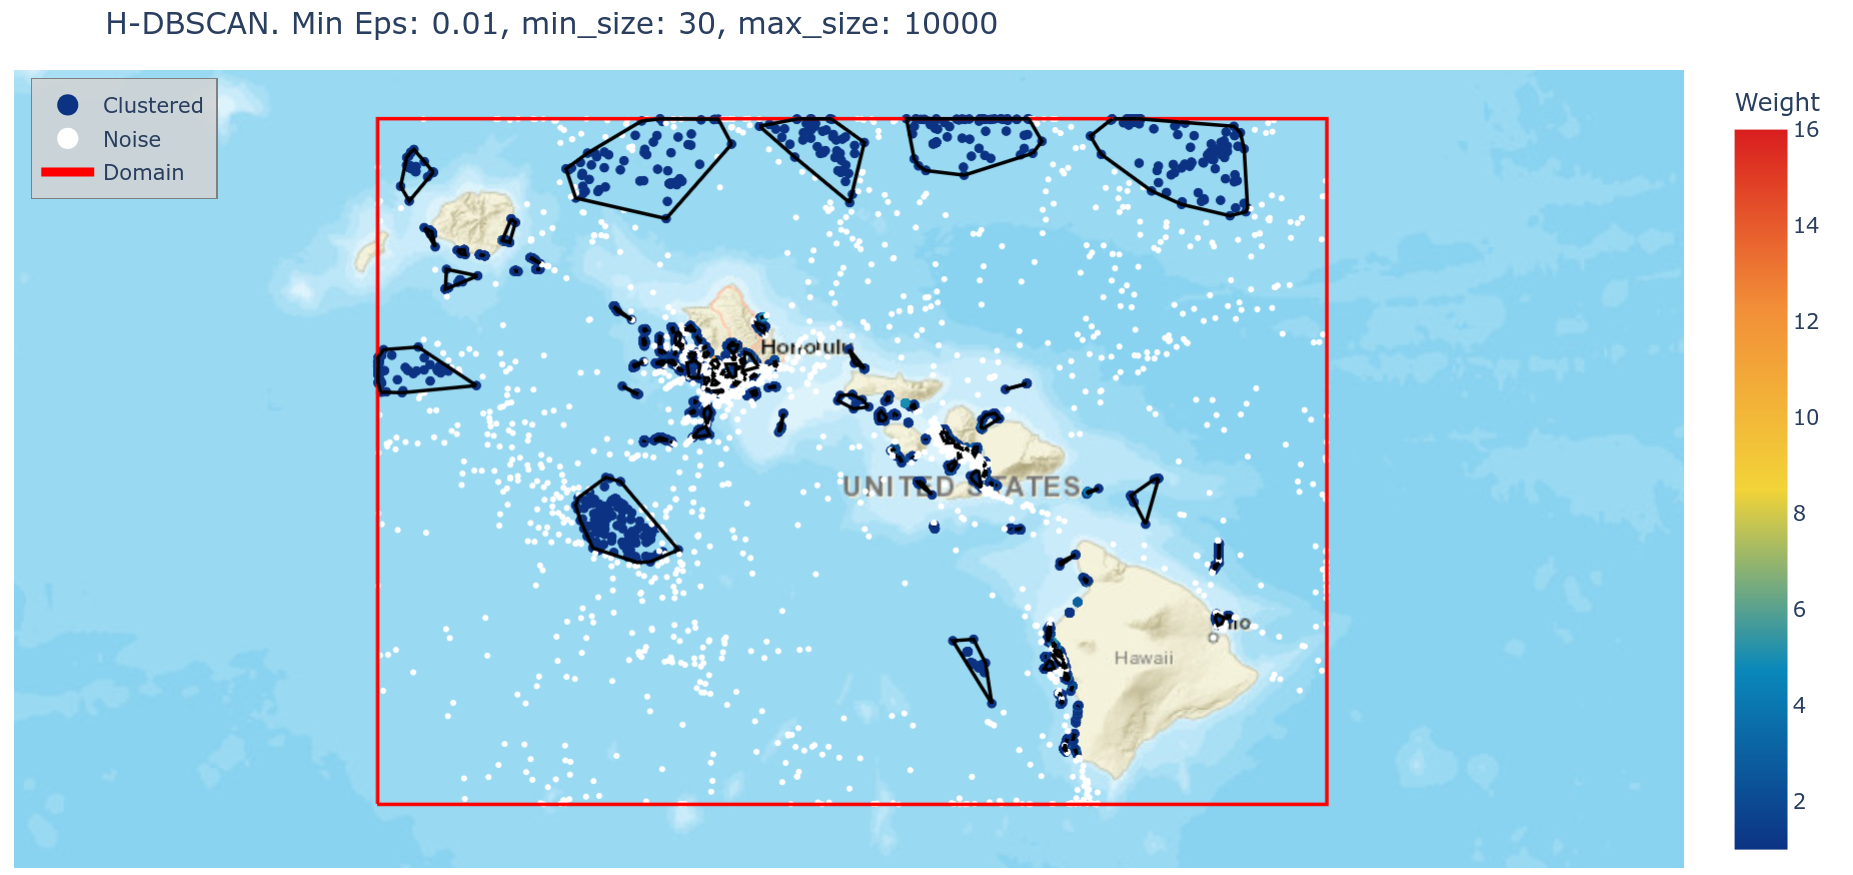
\includegraphics[width=\textwidth]{Results/H-DBSCAN.png}
    \caption{Waypoint identificati con H-DBSCAN ($\text{min\_cluster\_size} = 30$,
    $\text{max\_cluster\_size} = 10\,000$).}\label{fig:res_hdbscan}
\end{figure}

DBSCAN individua 55 cluster e classifica come rumore
1.001 delle 51.801 coordinate aggregate (1,93\%); H-DBSCAN, eseguito sulla tabella
espansa secondo i pesi (Sezione~\ref{ssec:meth_clustering}), individua 144 cluster e ne scarta 2.800 su 96.913
(2,89\%). Il confronto mette in evidenza il limite principale di DBSCAN con un raggio $\varepsilon$
fisso. Nell'area del porto di Honolulu e le zone di ancoraggio
vicine, la densità di punti stazionari è molto alta, e DBSCAN raggruppa tutta la zona in
un unico grande cluster che copre buona parte dell'isola. Lo stesso succede lungo la costa
occidentale dell'isola Maui e lungo la costa di Kona sull'isola di Hawaii, dove punti di sosta
distinti vengono fusi in poligoni allungati. Un waypoint di queste dimensioni non è utile
per l'estrazione delle rotte, perché fa coincidere in un solo nodo del grafo origini e
destinazioni che invece sono diverse.

H-DBSCAN, potendo adattarsi a densità locali diverse, scompone le stesse aree in molti
cluster più piccoli e compatti, che corrispondono in modo più plausibile a singoli porti,
moli e zone di ancoraggio. Nelle zone a bassa densità in mare aperto, invece, entrambi gli
algoritmi producono cluster di dimensioni simili (ad esempio il cluster a sud-ovest di Oahu
e quelli lungo il bordo settentrionale della bounding box). Per questo motivo H-DBSCAN è
stato adottato come approccio principale per le fasi successive della pipeline.

 
\subsection{Rotte estratte}
 
% PLACEHOLDER: inserire figura con la visualizzazione delle rotte estratte
% (grafo orientato waypoint → waypoint) sovrapposta alla mappa dell'arcipelago.
% Commentare le rotte principali emerse e la loro coerenza geografica.
 
\subsection{Trip sulla rotta selezionata}
 
% PLACEHOLDER: inserire figura con la visualizzazione dei 184 trip associati
% alla rotta selezionata WP_135 - WP_118.
 
% ─────────────────────────────────────────────
\section{Risultati quantitativi}\label{sec:res_quantitative}
 
\subsection{Parametri del modello Weibull}

I parametri della distribuzione di Weibull, stimati sull'intero insieme di 184 trip
della rotta selezionata (Sezione~\ref{sec:meth_anomaly}), risultano pari a
$m = 1{,}3105$ (coefficiente della relazione $\alpha = m \cdot \Delta t$ 
tra parametro di scala e intervallo temporale) e $\beta = 0{,}9358$ (parametro di forma medio).
 
% PLACEHOLDER: inserire grafico di fitting (shape/scale stimati sui vari lag
% temporali) a supporto dei valori riportati sopra.
 
\subsection{Anomaly scoring e ranking dei trip}
 
Applicando il modello ai 184 trip della rotta selezionata, i dieci trip con probabilità
combinata più alta (comportamento più regolare) sono, in ordine decrescente: i trip
23184, 24337, 23474, 8857, 11128, 14569, 8374, 15733, 25609 e 11307, con punteggi
compresi tra 3134,05 e 2534,98.
 
I dieci trip con probabilità combinata più bassa (candidati più probabili come
anomalie) sono, in ordine crescente di punteggio: il trip 3372 (211,39, il più
anomalo), seguito dai trip 3413, 3362, 10288, 30627, 10279, 24701, 7889, 30752
e 28433, con punteggi fino a 1196,21.
 
% PLACEHOLDER: inserire tabella riassuntiva con tutti i punteggi, e/o grafico
% della distribuzione dei punteggi sull'intera rotta.d
% PLACEHOLDER: inserire visualizzazione mappale dei trip con punteggio più
% basso sovrapposta a quella dei trip normali, per evidenziare visivamente
% le deviazioni.
 
\subsection{Metriche di valutazione}
 
% NOTA: le metriche quantitative non sono ancora state definite. Una volta
% stabilite, questa sottosezione dovrà riportare i valori ottenuti
% (es. AUC-ROC, precision/recall se disponibile un ground truth,
% oppure metriche interne come la separazione tra distribuzioni dei punteggi).
 
% ─────────────────────────────────────────────
\section{Interpretazione dei risultati}\label{sec:res_interpretation}
 
% PLACEHOLDER: questa sezione va scritta dopo aver ottenuto i risultati
% quantitativi. Di seguito alcune domande guida da affrontare:
%
% - I waypoint identificati corrispondono a porti, ancoraggi o punti di
%   passaggio noti dell'arcipelago? Ci sono waypoint inattesi?
% - Le rotte estratte riflettono le tratte commerciali o di traghetto
%   conosciute tra le isole?
% - I trip classificati come più anomali presentano caratteristiche
%   interpretabili (deviazioni spaziali, velocità inusuali, durate anomale)?
% - In che misura i risultati sono confrontabili con quelli riportati da
%   Pallotta et al. nel loro dataset originale (Stretto di Gibilterra,
%   Adriatico settentrionale)?
 
% ─────────────────────────────────────────────
\section{Sintesi}\label{sec:res_summary}
 
% PLACEHOLDER: scrivere dopo aver completato le sezioni precedenti.
% La sintesi dovrà riprendere brevemente i risultati principali e
% anticipare il Capitolo~\ref{chap:conclusions}, in cui verranno discusse
% le conclusioni generali e le possibili direzioni future.


% Conclusions
% sections/conclusions.tex
\chapter{Conclusions}
\label{chap:conclusions}

Conclusioni, in cui indico in che modo il mio lavoro ha portato delle migliorie
ed eventualmente quali aspetti possono/devono essere ancora esplorati/approfonditi

\section{Sezione 1 - Sintesi dei contributi principali}
Testo Sezione 1

\section{Sezione 2 - Migliorie ottenute}
Testo sezione 2

\section{Sezione 3 - Limititazioni/difetti}
Testo sezione 3

\section{Sezione 4 - Sviluppi futuri}
Testo Sezione 4

\section{Sezione 5 - Conclusione finale}


% Bibliography
%\nocite{*} %adds all bibliography to the main file
\bibliographystyle{unsrtnat}
\bibliography{bibliography}

% Appendices (if any)
\appendix
% \input{sections/appendices}

\end{document}
